\documentclass[12pt,letterpaper]{article}   % Tamaño 12, papel carta

% Paquetes esenciales
\usepackage[spanish]{babel}        % Idioma español
\usepackage[utf8]{inputenc}        % Codificación UTF-8
\usepackage[T1]{fontenc}           % Codificación de fuente
\usepackage{setspace}              % Control del interlineado
\usepackage[margin=2.5cm]{geometry}% Márgenes de 2.5cm
\usepackage{parskip}               % Evita sangrías y añade espacio entre párrafos

\usepackage{graphicx}              % Para incluir imágenes 
\usepackage{titling}               % Para personalizar la portada
\usepackage{amsmath}               % Para mates
\usepackage{amssymb}               % Letras de mates
\usepackage{hyperref}              % Para el índice

\usepackage{amsfonts}
\usepackage{pgfplots}
\usepackage{booktabs}

% Interlineado 1.5
\onehalfspacing

% Justificación del texto
\usepackage{ragged2e}
\justifying

% No sangría en párrafos
\setlength{\parindent}{0pt}

% Numerado de pagina arriba a la derecha
\usepackage{fancyhdr}
\pagestyle{fancy}
\fancyhf{} % Limpia encabezados y pies predeterminados
\fancyhead[R]{\thepage} % Número de página en encabezado derecha
\renewcommand{\headrulewidth}{0pt} % Elimina la línea bajo el encabezado

% Que los titulos de las secciónes tengan el mismo tamaño
\usepackage{titlesec}

% Configuración de \section
\titlespacing*{\section}{0pt}{2ex plus 1ex minus .2ex}{-0.5ex} 
\titleformat{\section}[block]{\normalfont\normalsize\bfseries}{\thesection}{1em}{}

\titlespacing*{\subsection}{0pt}{2ex plus 1ex minus .2ex}{-0.5ex} 
\titleformat{\subsection}[block]{\normalfont\normalsize\bfseries}{\thesubsection}{1em}{}

\titlespacing*{\subsubsection}{0pt}{2ex plus 1ex minus .2ex}{-0.5ex} 
\titleformat{\subsubsection}[block]{\normalfont\normalsize\bfseries}{\thesubsubsection}{1em}{}

\titlespacing*{\paragraph}{0pt}{2ex plus 1ex minus .2ex}{-0.5ex} 
\titleformat{\paragraph}[block]{\normalfont\normalsize\bfseries}{\paragraph}{1em}{}

\titlespacing*{\subparagraph}{0pt}{2ex plus 1ex minus .2ex}{-0.5ex} 
\titleformat{\subparagraph}[block]{\normalfont\normalsize\bfseries}{\subparagraph}{1em}{}


% Consola
\usepackage{listings}
\usepackage{xcolor}
\definecolor{consolegray}{gray}{0.95}
\definecolor{consoleborder}{gray}{0.7}
\lstnewenvironment{smallconsole}[1][]{
  \lstset{
    basicstyle=\ttfamily\tiny, 
    backgroundcolor=\color{consolegray},
    frame=single,
    rulecolor=\color{consoleborder},
    breaklines=true,
    columns=fullflexible,
    showstringspaces=false,
    captionpos=b,
    xleftmargin=1em,
    xrightmargin=1em,
    aboveskip=1em,
    belowskip=1em,
    #1 % ← Para pasar opciones como caption
  }
}{}


% Tamaño de las captions
\usepackage{caption}
\captionsetup{font=scriptsize}

% Multicolumnas
\usepackage{multicol}
\usepackage{listings}
\usepackage{xcolor}
\usepackage{multicol}

\definecolor{consolegray}{gray}{0.95}
\definecolor{consoleborder}{gray}{0.7}

% Define el estilo una vez
\lstdefinestyle{smallconsolestyle}{
  basicstyle=\ttfamily\tiny,
  breaklines=true,
  columns=fullflexible,
  showstringspaces=false,
  captionpos=b,
  xleftmargin=0em,
  xrightmargin=0em,
  aboveskip=1em,
  belowskip=1em,
  frame=none,
  backgroundcolor=\color{white},
  rulecolor=\color{white}
}




% Configuración para usar el punto como separador decimal
\renewcommand{\theequation}{\arabic{equation}}



\begin{document}




% ----------------------------------
% Portada
% ----------------------------------
\begin{titlepage}
    \begin{center}
        \vspace*{2cm}
        \textbf{Portafolios para Criptomonedas}\\[2cm]

        Heriberto Espino Montelongo - 175199\\[0.5cm]
        Universidad de las Américas Puebla\\[0.5cm]
        P25 LDS1131 1: Visualización de Datos\\[0.5cm]
        Dr. Hector Saib Maravillo Gomez\\[0.5cm]
        12 de mayo de 2025\\
    \end{center}
    \vfill
\end{titlepage}


% ----------------------------------
% Contenido del documento
% ----------------------------------


\pagenumbering{Roman}
\setcounter{page}{1}
\tableofcontents
\newpage



% A partir de aquí empieza la numeración arábiga desde 1
\pagenumbering{arabic}
\setcounter{page}{1}




\section{Introducción}
\subsection{Contextualización y relevancia del problema abordado}
Durante la última década, el ecosistema de criptoactivos ha presentado un crecimiento sin precedentes, alcanzando una capitalización superior a los 2 billones de dólares para comienzos de 2025 (CoinMarketCap, 2025). Esta expansión ha transformado profundamente el perfil de los participantes del mercado, incluyendo tanto actores institucionales como inversores minoristas. Lo anterior ha generado una demanda creciente por metodologías analíticas rigurosas orientadas a la evaluación del binomio riesgo-retorno (Fisch et al., 2019). La presencia de productos derivados, tokens con diversas funciones, y ecosistemas interconectados ha hecho indispensable el uso de enfoques cuantitativos robustos y adaptativos.

La inherente volatilidad de los precios, la diversidad funcional de los activos digitales y su interconectividad creciente exigen un enfoque integral basado en ciencia de datos. Este enfoque debe combinar herramientas cuantitativas avanzadas, técnicas de visualización interpretativa, y principios de diseño perceptual. Es crucial tener una comprensión dinámica de la estructura del mercado y de los factores que influyen en el comportamiento de los criptoactivos (Liu et al., 2022). En este contexto, el presente trabajo busca aportar una caracterización multidimensional de un portafolio de criptoactivos representativo del ecosistema actual, con énfasis en optimización, simulación y análisis estructural.

\subsection{Delimitación temporal, espacial y conceptual del estudio}
Este estudio se centra en el período de mayo de 2024 a mayo de 2025, seleccionado por su relevancia en cuanto a dinamismo del mercado y cambios estructurales recientes en el ecosistema cripto (Messari, 2025). Esta etapa incluye hitos regulatorios clave, lanzamientos tecnológicos, e importantes movimientos en el comportamiento de precios y volúmenes. La muestra incluye una selección de criptoactivos clasificados conforme a criterios de capitalización bursátil, funcionalidad tecnológica y relevancia dentro del ecosistema cripto:

\begin{enumerate}
\item Activos de alta capitalización: BTC, ETH, USDT, BNB, USDC, XRP, ADA, SOL, DOGE (CoinGecko, 2025).
\item Stablecoins de referencia: USDT, USDC, DAI, USDS (MakerDAO, 2024).
\item Tokens de infraestructura blockchain: TRX, TON, MATIC, DOT, AVAX, STETH, WSTETH, SUI (Electric Capital, 2025).
\item Activos envueltos para interoperabilidad: WBTC, WTRX, WSTETH (BitGo, 2025).
\item Criptoactivos con uso en pagos y DeFi: LTC, LINK, XLM, HBAR, BCH (DeFiLlama, 2025).
\item Memecoins con tracción social: DOGE, SHIB (Santiment, 2024).
\item Tokens asociados a exchanges: LEO (Bitfinex, 2025).
\end{enumerate}

Se comparan mecanismos de exposición directa (spot) y derivados financieros (CFDs), considerando su eficiencia, perfiles de riesgo y comportamiento bajo escenarios empíricos y simulados. El marco espacial presupone plataformas de negociación globalizadas con precios denominados en dólares estadounidenses. El marco conceptual abarca teoría de optimización de portafolios (Markowitz, 1952), procesos estocásticos (GBM) y análisis estructural de interdependencias mediante redes financieras (Mantegna, 1999).

\subsection{Objetivos del estudio}
Los objetivos específicos comprenden:
\begin{itemize}
\item Evaluar eventos clave del ecosistema cripto y su efecto sobre activos seleccionados como BTC, ETH, DOGE y XRP, tanto en precio como en volumen.
\item Caracterizar correlaciones y patrones de agrupamiento entre activos a partir de log-retornos.
\item Formular y contrastar portafolios optimizados (spot y CFD) mediante la frontera eficiente de Markowitz.
\item Simular trayectorias de precios a corto plazo utilizando Movimiento Browniano Geométrico (GBM) con parámetros calibrados empíricamente.
\end{itemize}

\section{Metodología}
\subsection{Herramientas analíticas y técnicas de ciencia de datos implementadas}
El abordaje metodológico incluyó:
\begin{itemize}
\item Optimización: programación cuadrática para construir la frontera eficiente de Markowitz.
\item Modelado estocástico: generación de trayectorias a 30 días mediante Movimiento Browniano Geométrico (GBM), calibrado por volatilidad histórica.
\item Correlaciones: coeficientes de Pearson sobre log-retornos diarios; disimilitud definida como $d_{ij}=1-\left|\rho_{ij}\right|$. % (Tumminello et al., 2005).
\item Clustering y redes: mapas jerárquicos, clústeres de activos y grafos construidos con visualización mediante Kamada-Kawai de\texttt{networkx}.
% \item Análisis de eventos: evaluación de shocks tecnológicos, regulatorios y sociales sobre comportamiento de precios y volumen (Chainalysis, 2024).
\end{itemize}

\subsection{Origen y tratamiento de los datos}
Se utilizaron series diarias de precios y volúmenes extraídas desde la API pública de Yahoo Finance, en el intervalo mayo 2024 - mayo 2025 (Yahoo Finance, 2025). Las etapas incluyeron:
\begin{enumerate}
\item \textbf{Extracción}: adquisición automatizada del precio ajustado y volumen diario mediante \texttt{yfinance}.
\item \textbf{Preprocesamiento}: validación de completitud; no fue necesario imputar datos.
\item \textbf{Transformación}: cálculo de log-retornos para estabilizar varianza y mejorar la idoneidad del modelado estocástico (Cont, 2001).
\item \textbf{Análisis exploratorio}: estimación preliminar de correlaciones y volúmenes relativos.
\end{enumerate}

\section{Resultados}
\subsection{Resultados analíticos y representación visual}


\subsubsection{Análisis de áctivos}
Del análisis de criptoactvos, se pueden concluir que estos actitvos son altamnente sensibles a eventos sociales y tecnológicos. En la figura \ref{fig:1} se puede observar el comportamiento de los precios y volumen de los activos más populares durante el último año.

\begin{figure}[h!]
    \centering
    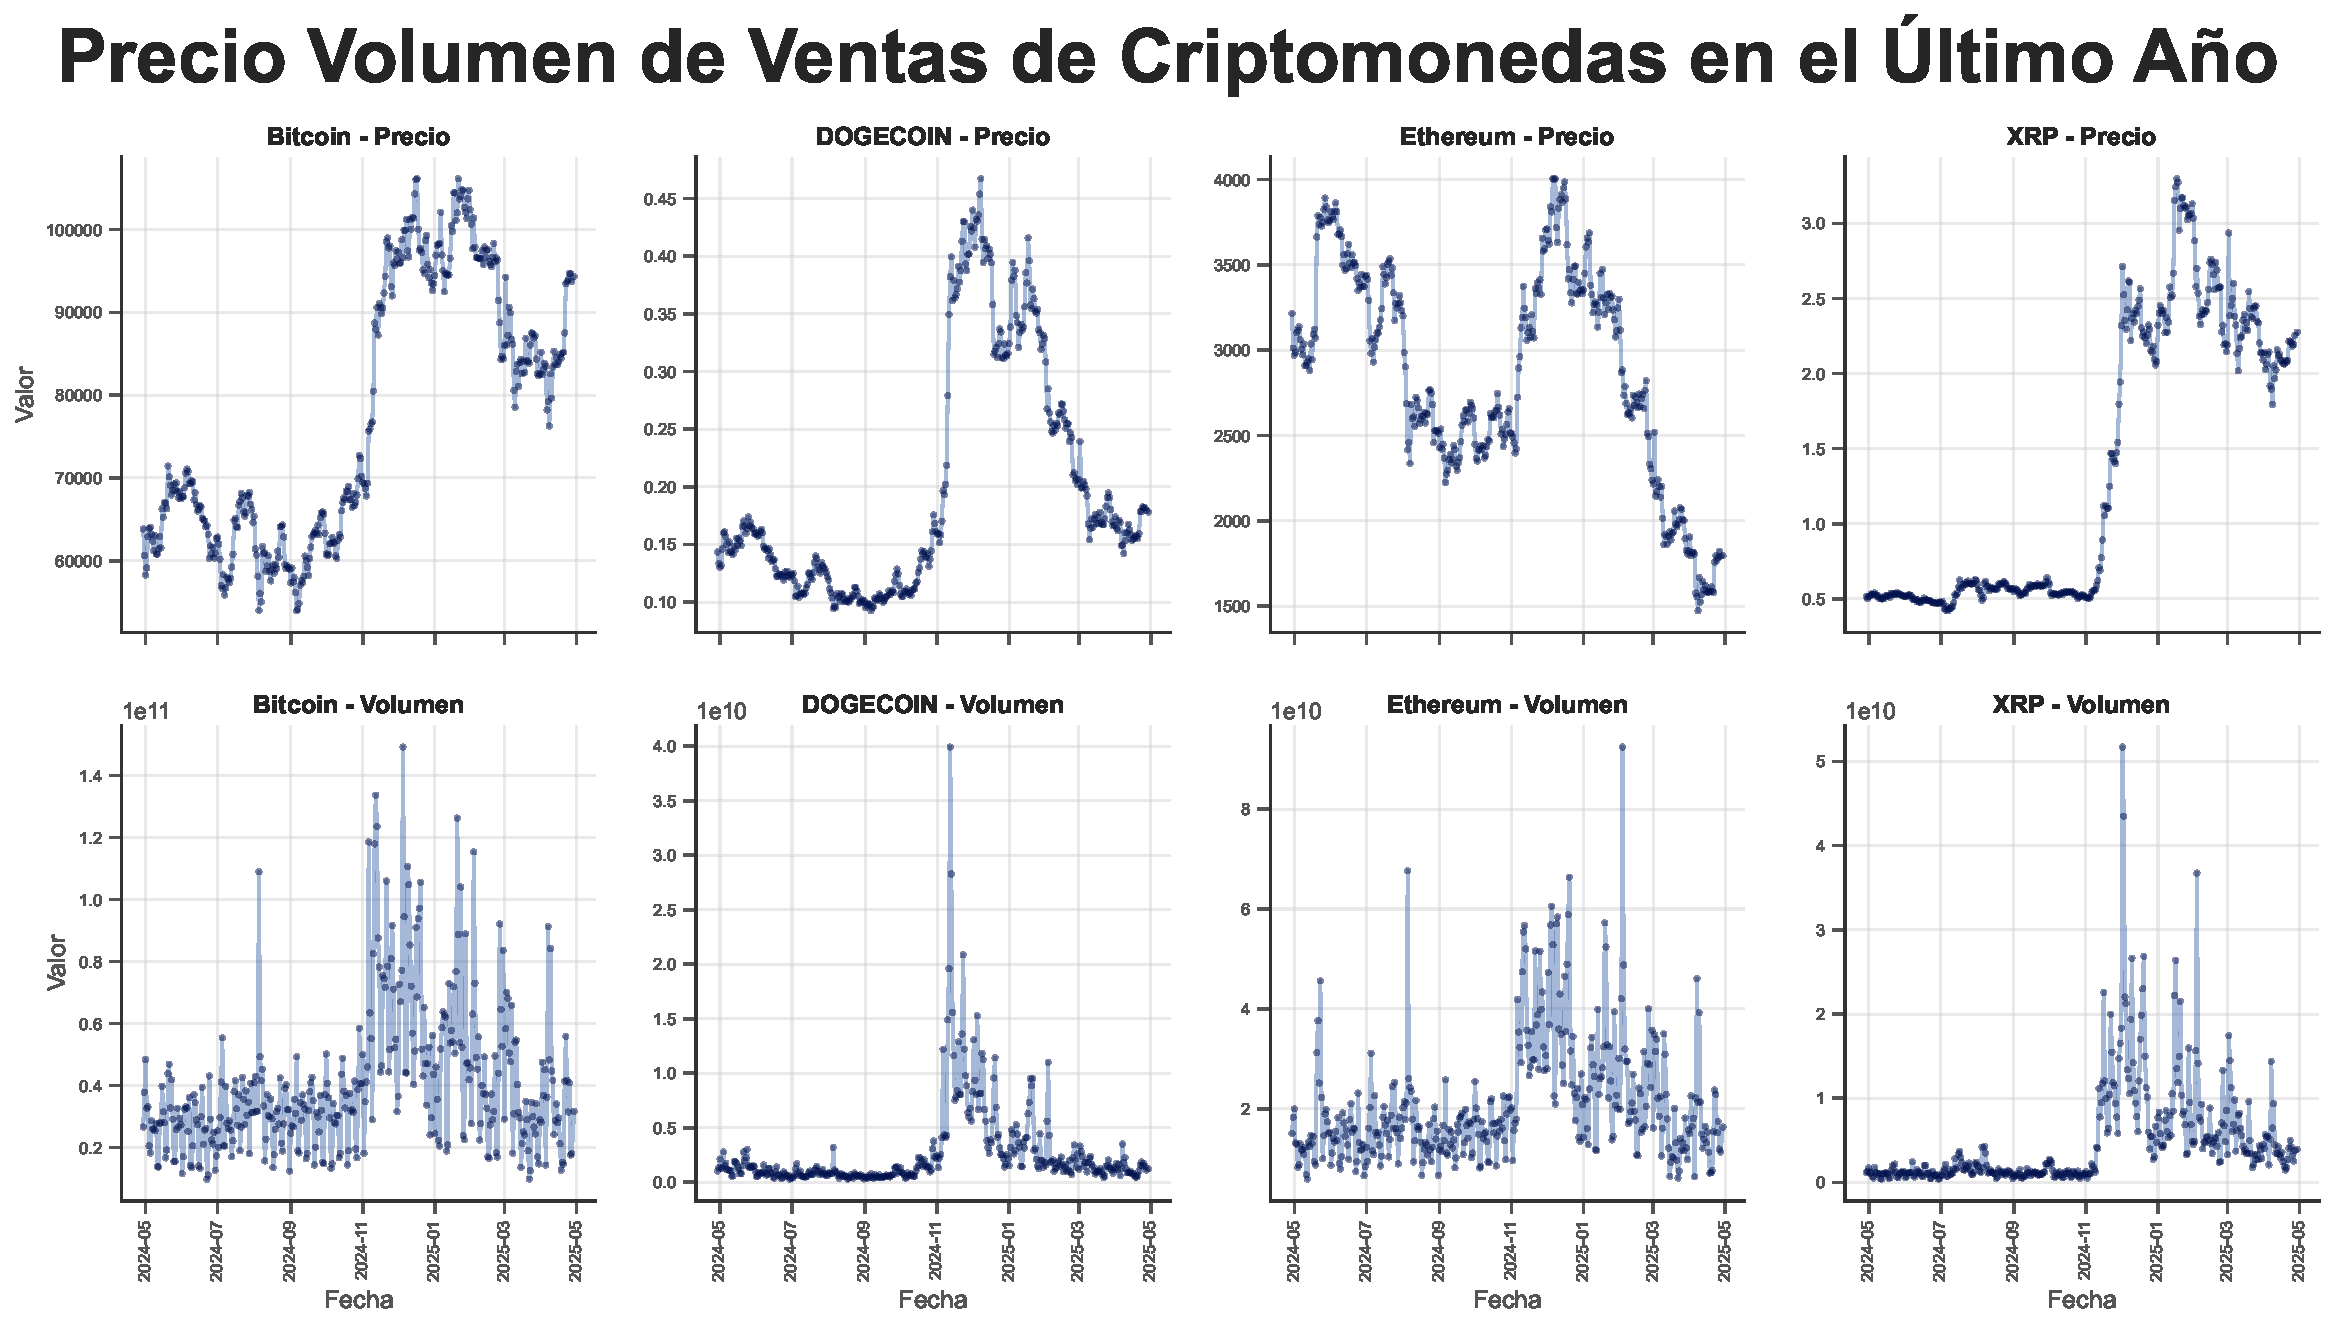
\includegraphics[width=0.85\textwidth]{imagenes/09-Precio-Volumen.pdf}
    \caption{\textit{Elaboración Propia}. Descripción de la imagen.}
    \label{fig:1}
\end{figure}




\subsubsection{Análisis de Correlaciones}

La matriz de correlación reveló interdependencias predominantemente positivas. TON, DAI y LEO se identificaron como activos con baja correlación estructural, lo que sugiere su rol como activos diversificadores potenciales. La visualización mediante el algoritmo Kamada-Kawai resaltó estas relaciones. % (Kenett et al., 2010)





\begin{figure}[h!]
    \centering
    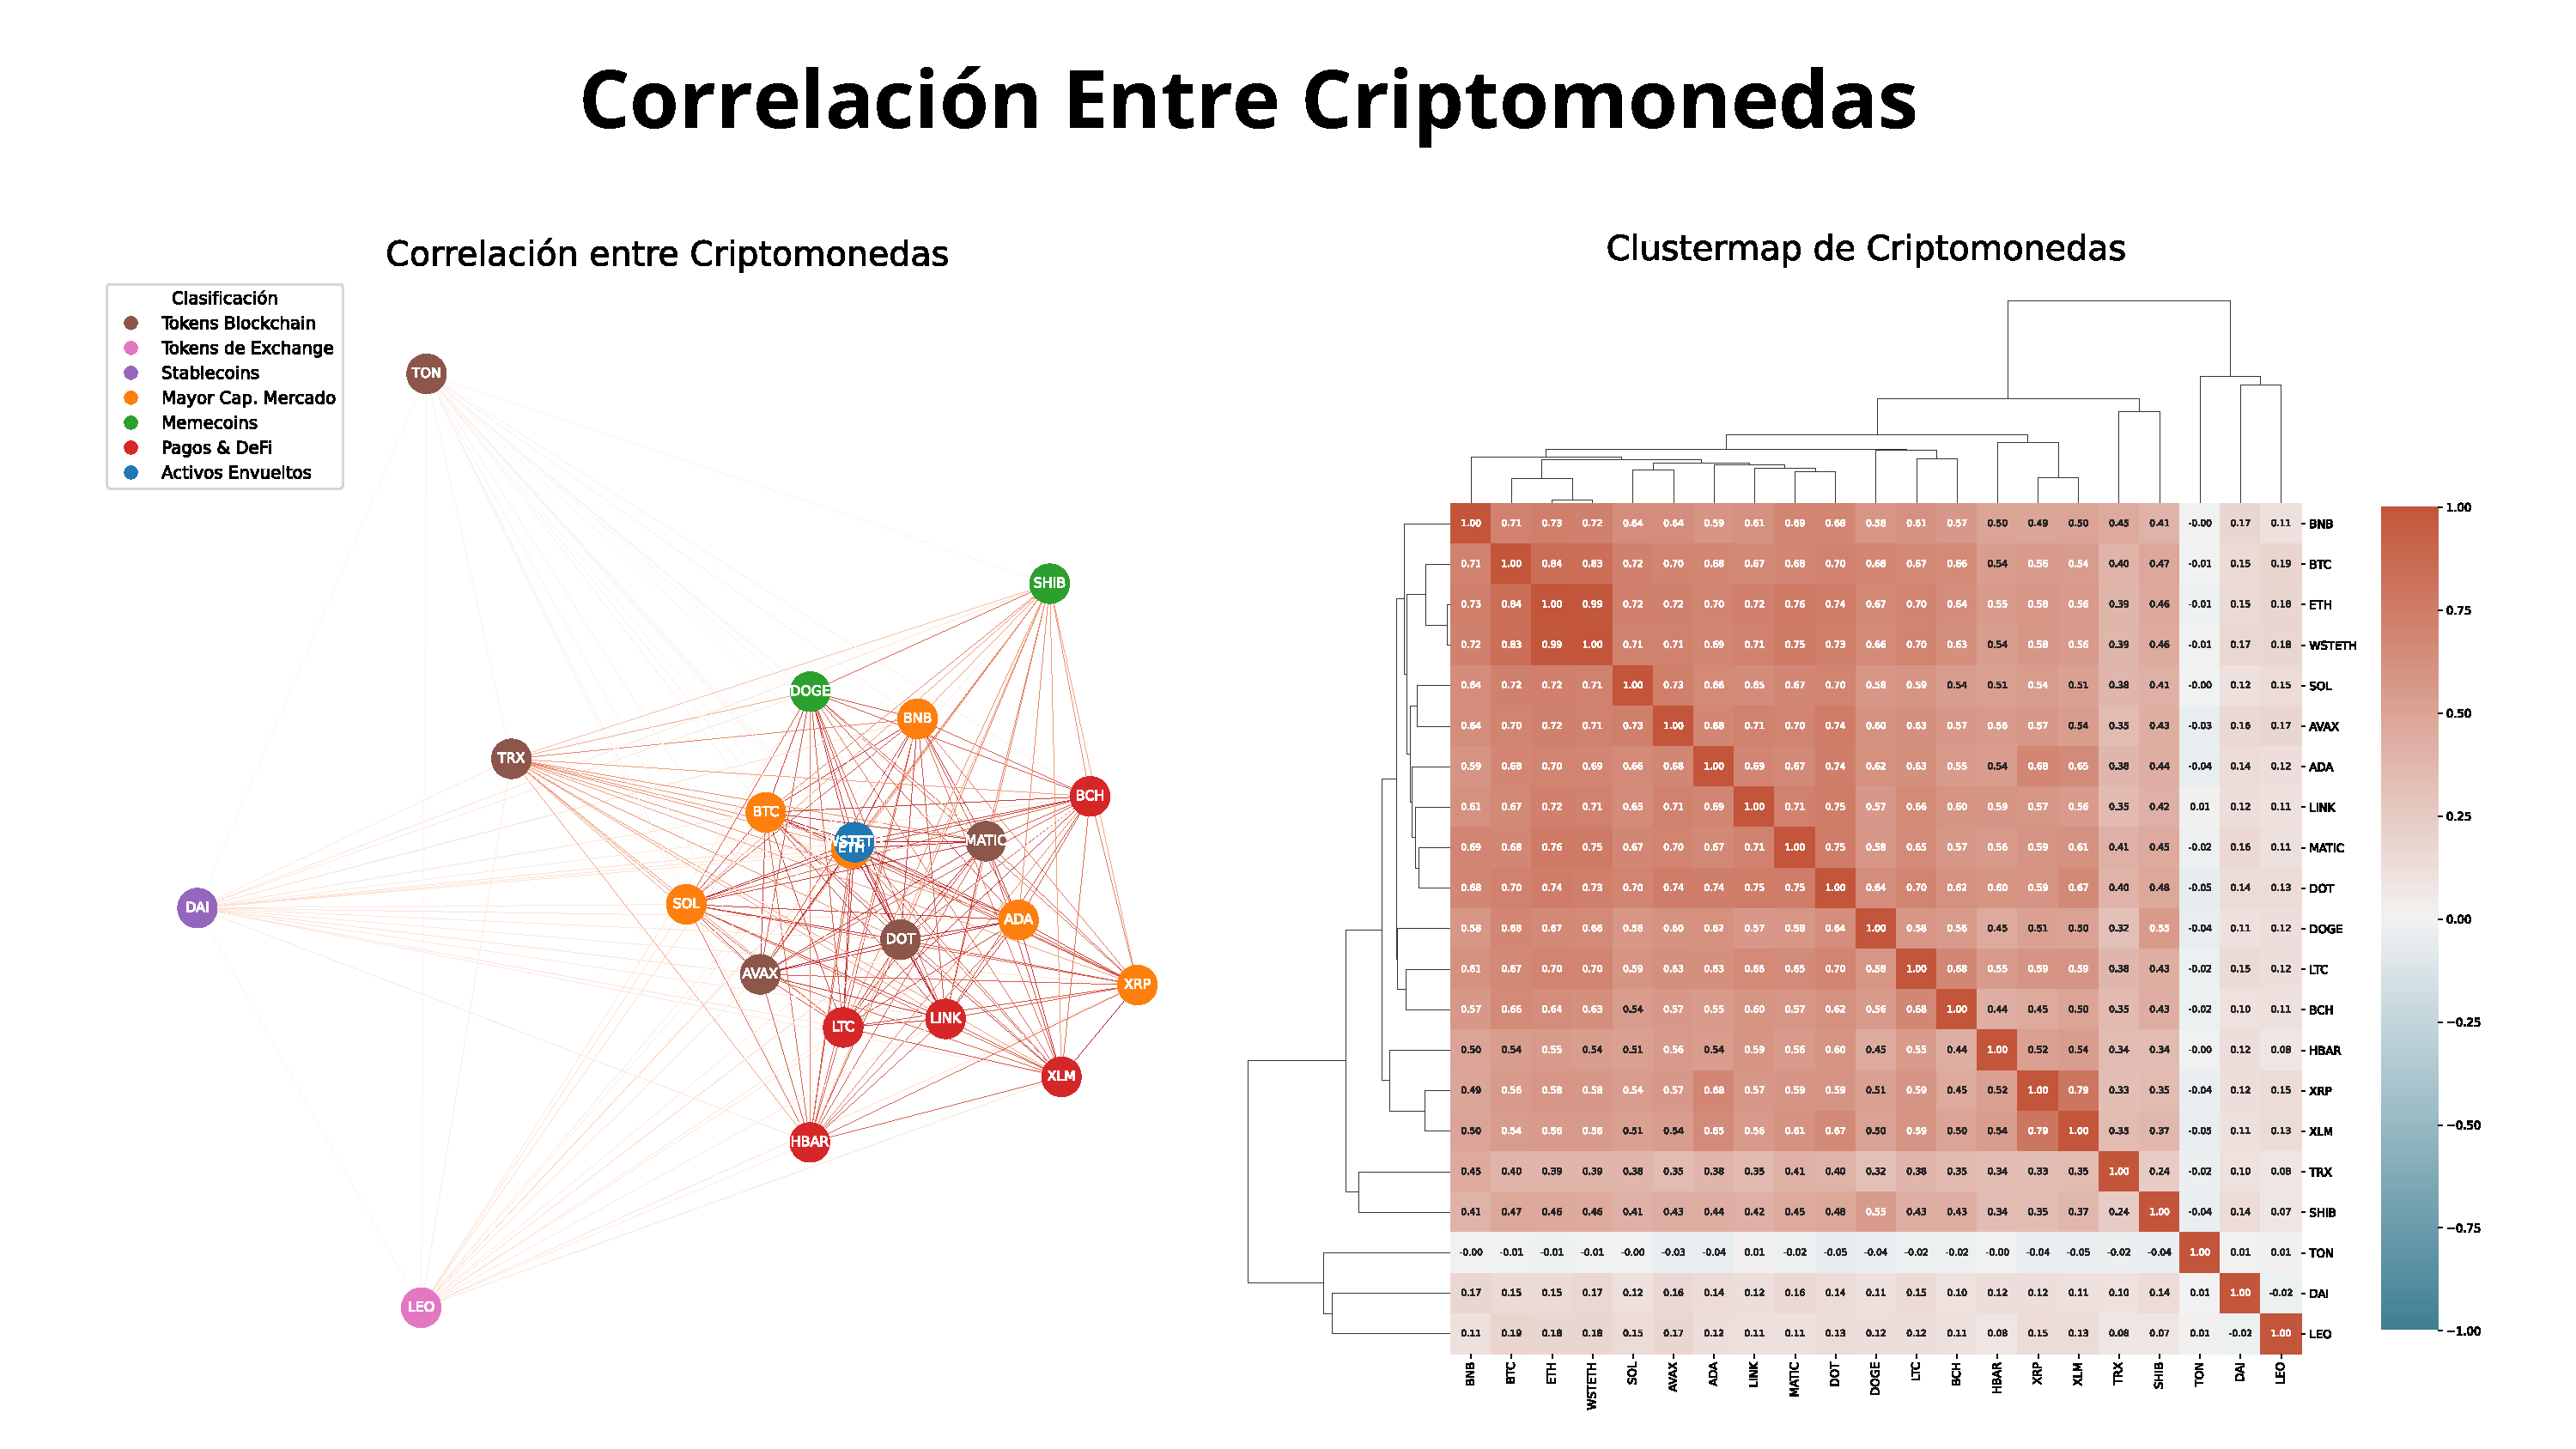
\includegraphics[width=0.9\textwidth]{imagenes/10-Correlacion-Entre-Criptomonedas.pdf}
    \caption{\textit{Elaboración Propia}. Descripción de la imagen.}
    \label{fig:mi_imagen}
\end{figure}




\subsubsection{Curvas de frontera eficiente}


\begin{figure}[h!]
    \centering
    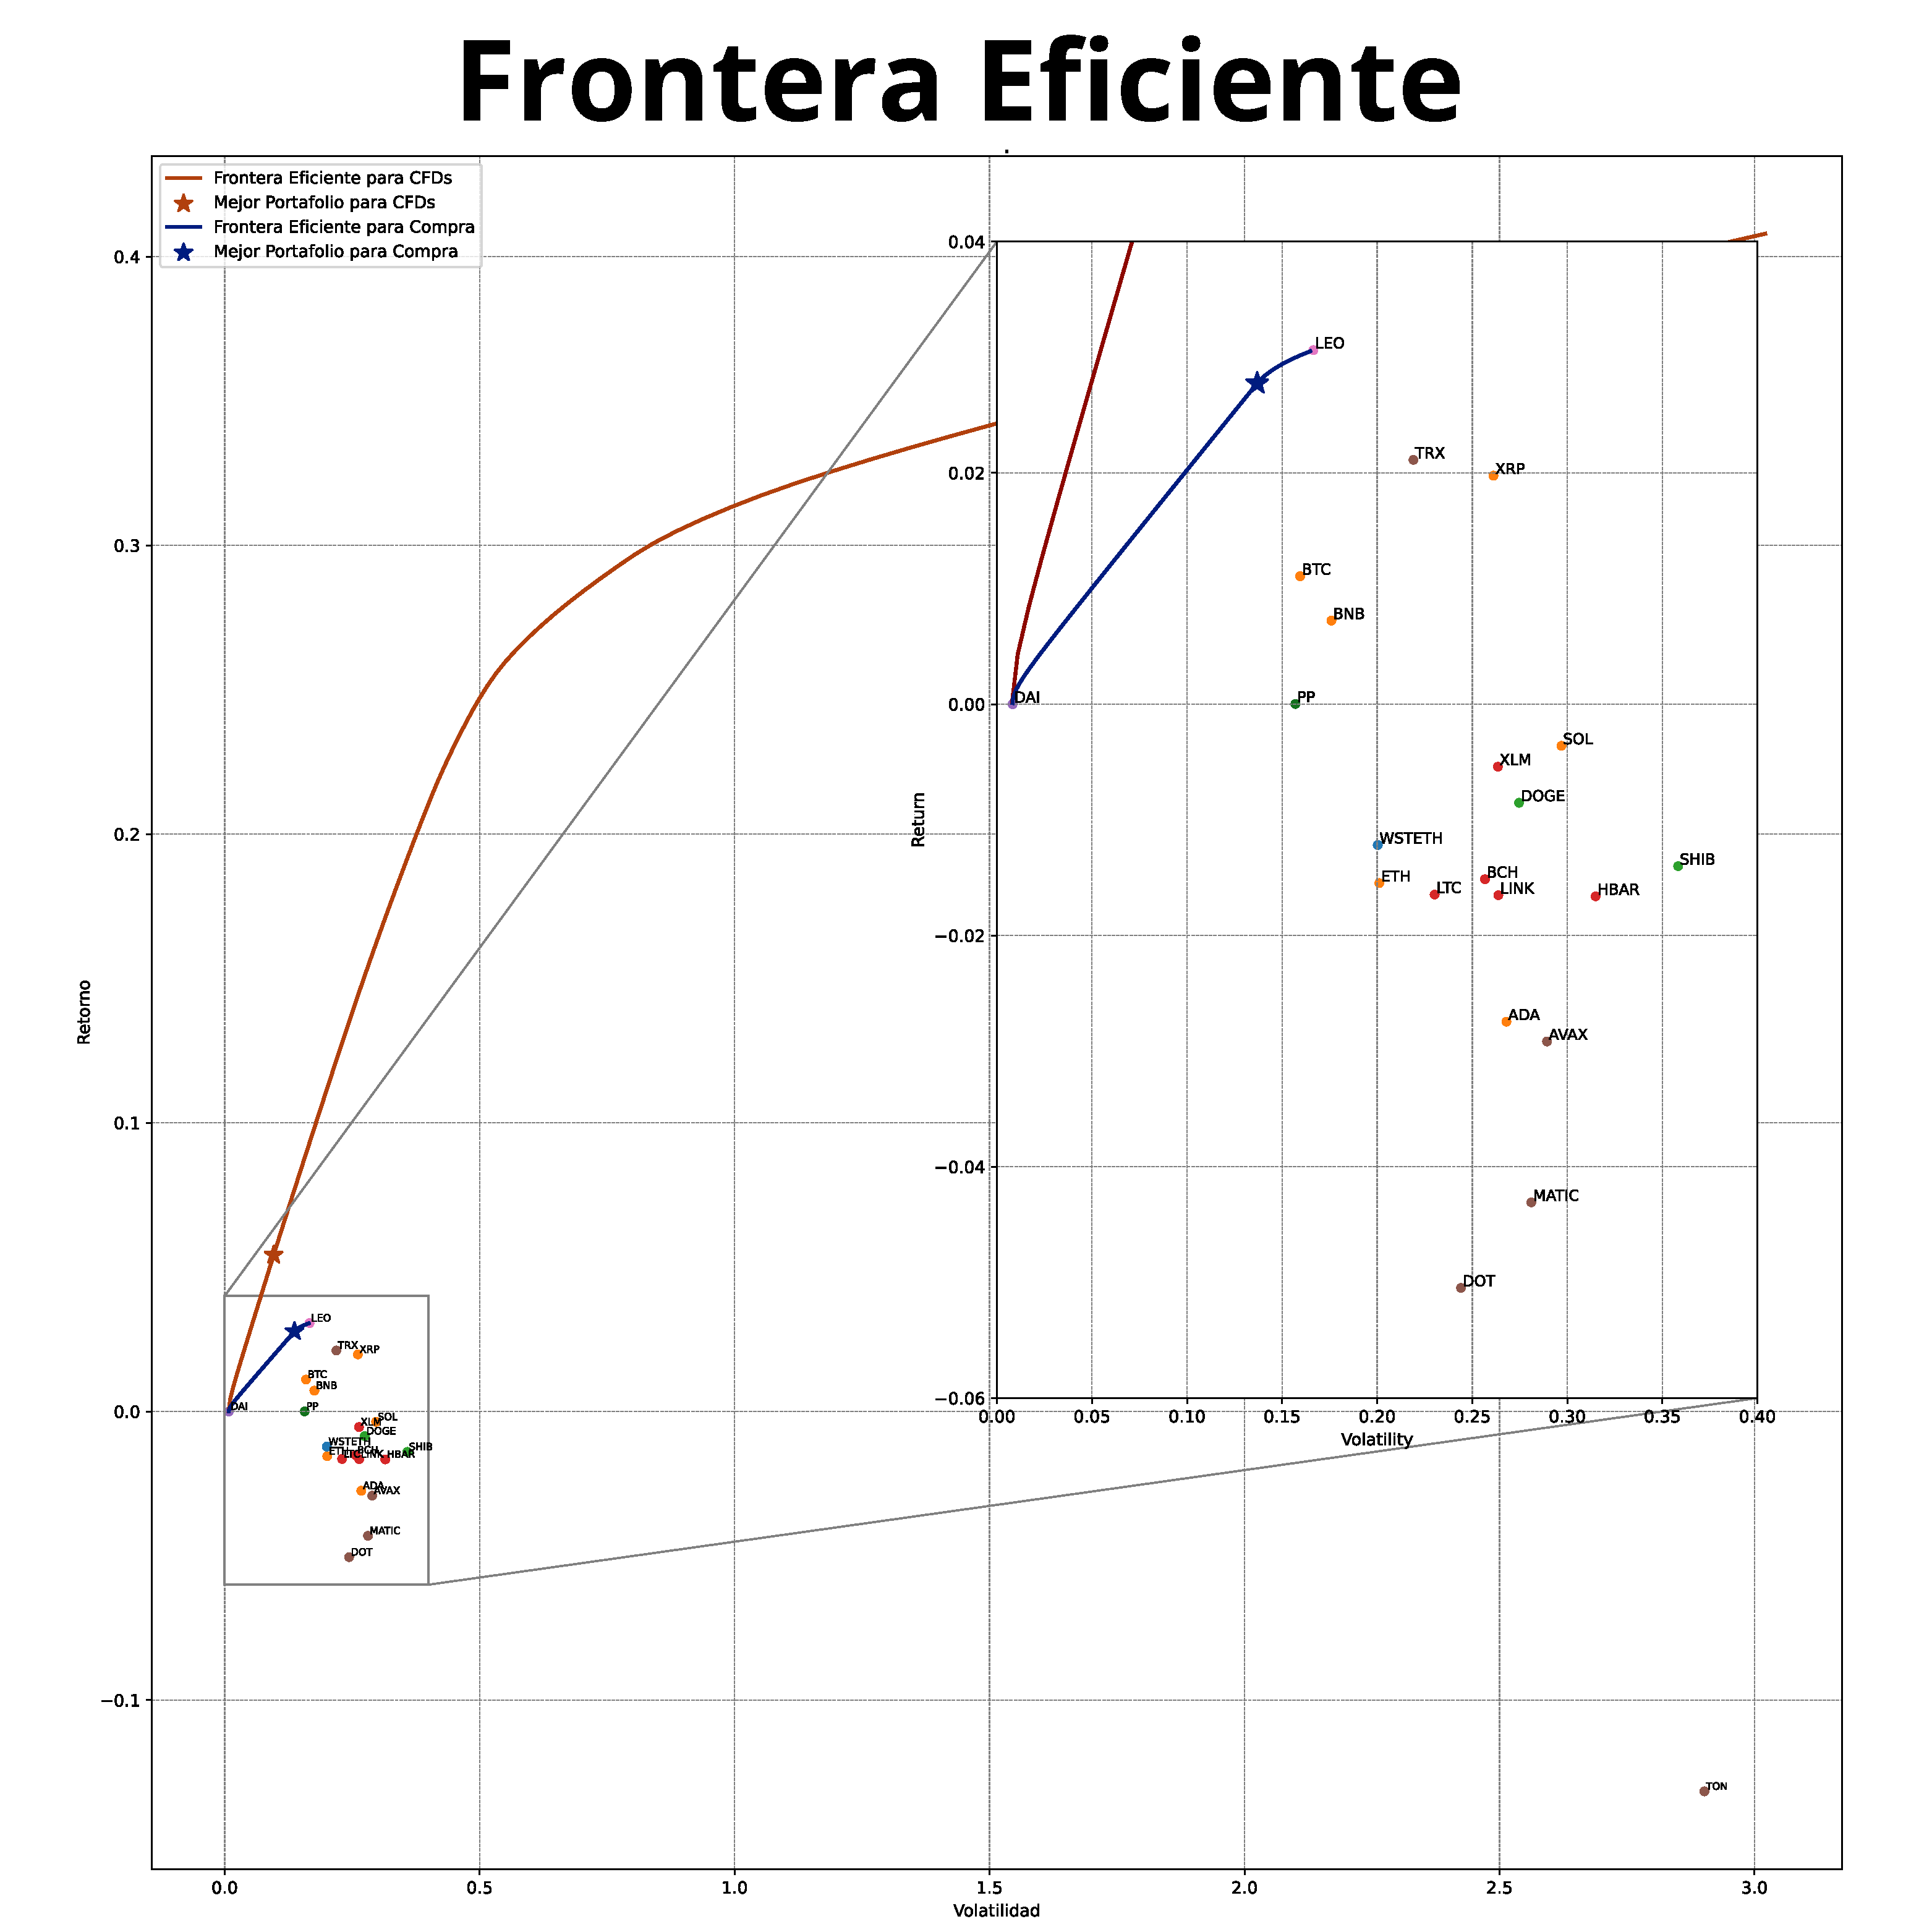
\includegraphics[width=0.55\textwidth]{imagenes/10-ef.pdf}
    \caption{\textit{Elaboración Propia}. Descripción de la imagen.}
    \label{fig:mi_imagen}
\end{figure}

Dos portafolios eficientes fueron generados (Figura fig:peso). El portafolio spot presentó diversificación moderada entre activos, mientras que el de CFDs evidenció concentración marcada en activos de alta volatilidad como DOGE (Zhang et al., 2023). En términos de retorno esperado y riesgo, ambos portafolios superaron el benchmark pasivo, aunque el CFD mostró una varianza esperada sustancialmente mayor, implicando mayor riesgo.



\newpage


\subsubsection{Simulaciones de Monte Carlo con Movimiento Browniano Geométrico}

Las simulaciones GBM a 30 días mostraron trayectorias divergentes. El portafolio CFD evidenció colas pesadas y escenarios extremos de ganancia o pérdida total. El portafolio spot mostró un comportamiento más simétrico, con mayor estabilidad y menor dispersión, aunque ambos presentaron rendimientos esperados positivos (Hull, 2015).

\begin{figure}[h!]
    \centering
    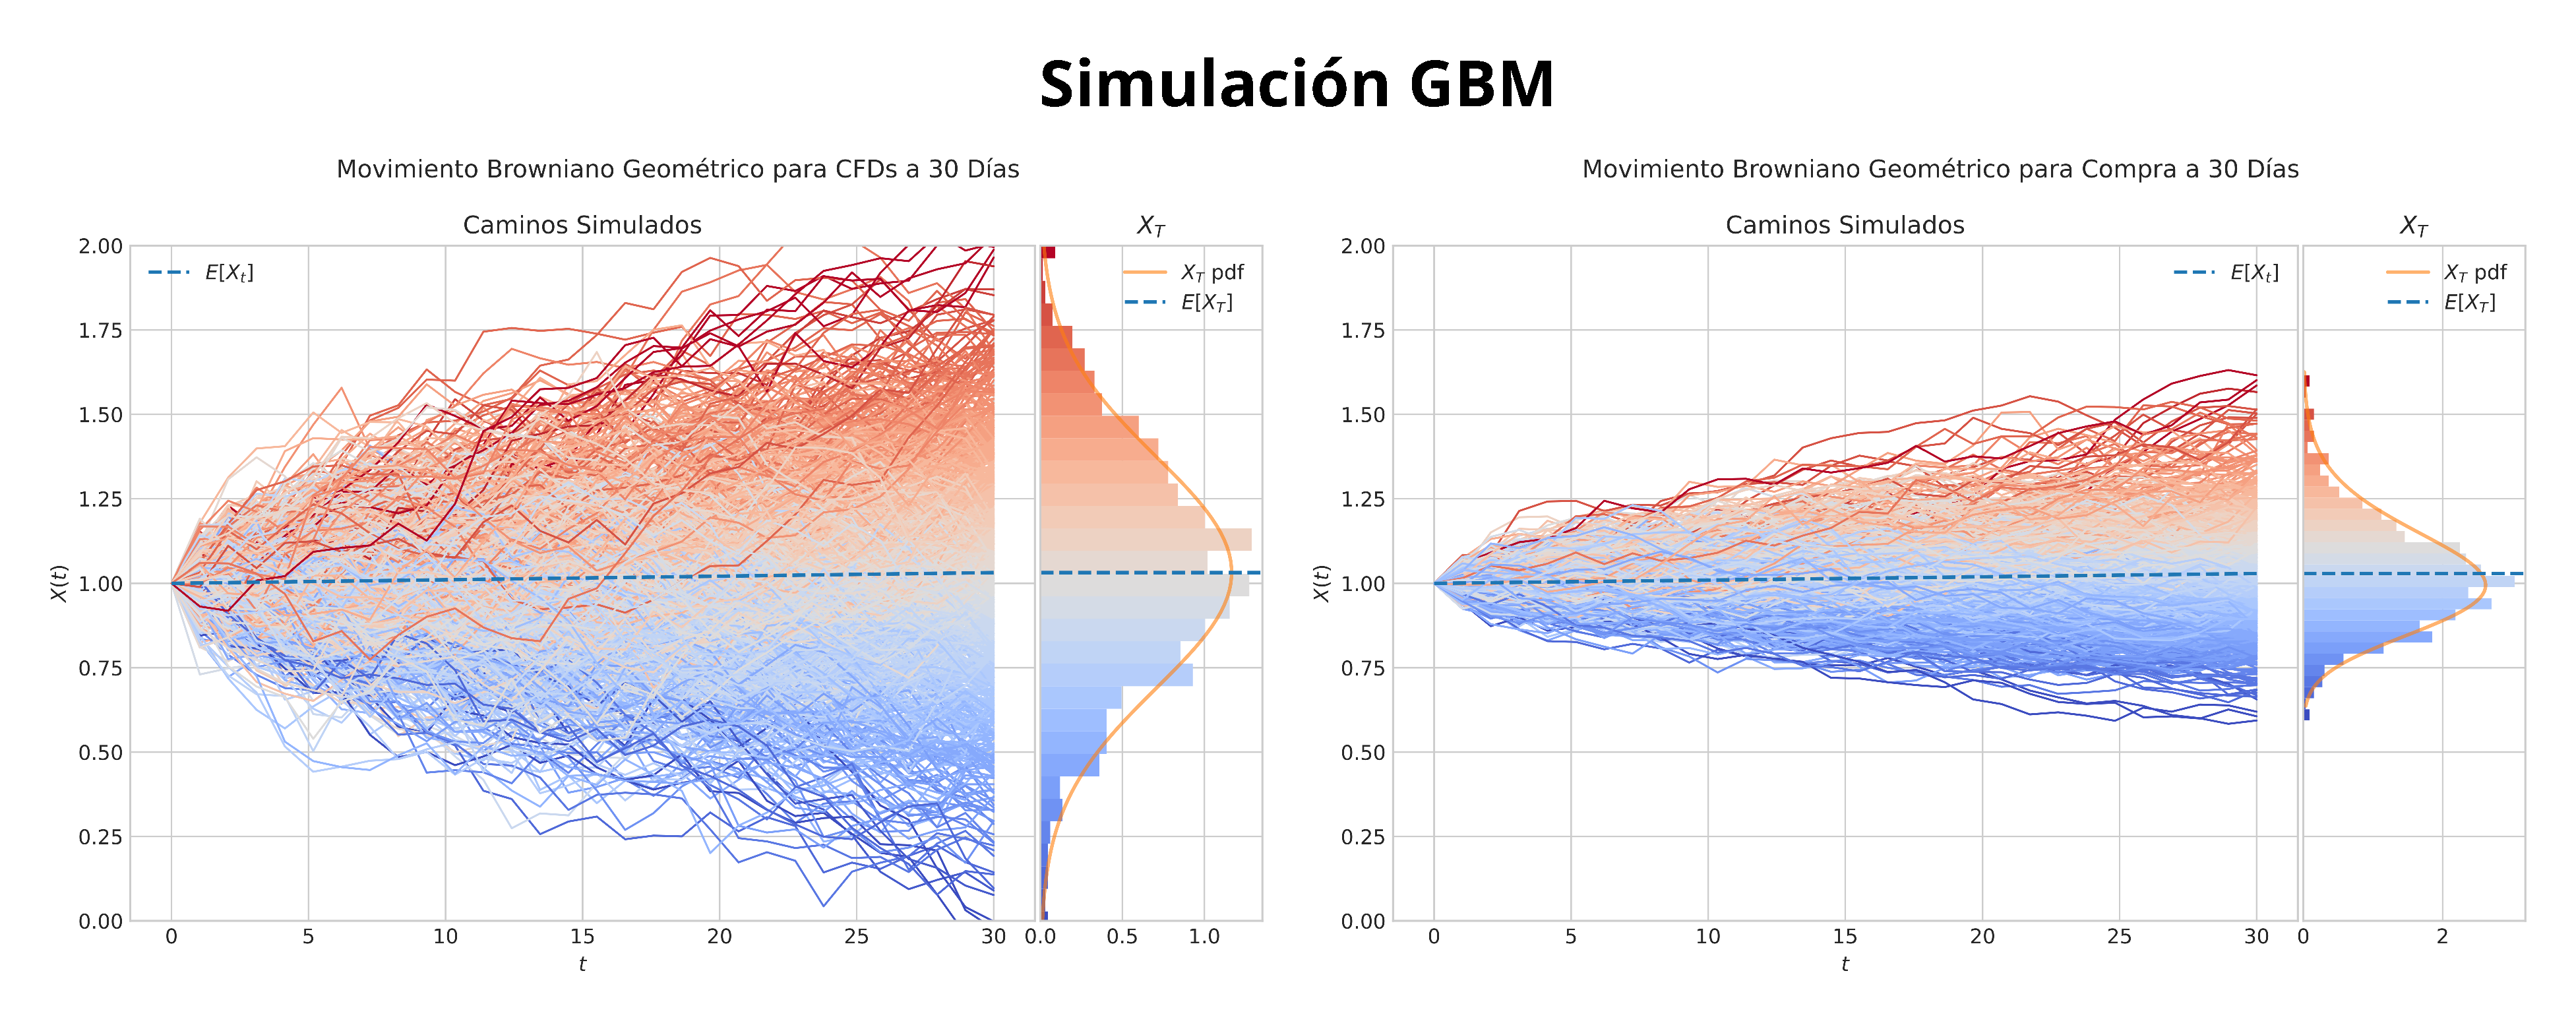
\includegraphics[width=1\textwidth]{imagenes/10-Simulacion-GBM-h.pdf}
    \caption{\textit{Elaboración Propia}. Descripción de la imagen.}
    \label{fig:mi_imagen}
\end{figure}




\subsection{Visualización de hallazgos mediante paneles gráficos}
Se implementaron dashboards visuales que incluyen asignación de pesos, trayectorias GBM, scatterplots riesgo-retorno, clustermaps de correlaciones, grafos de similitud estructural y análisis multievento.
\begin{figure}[h!]
    \centering
    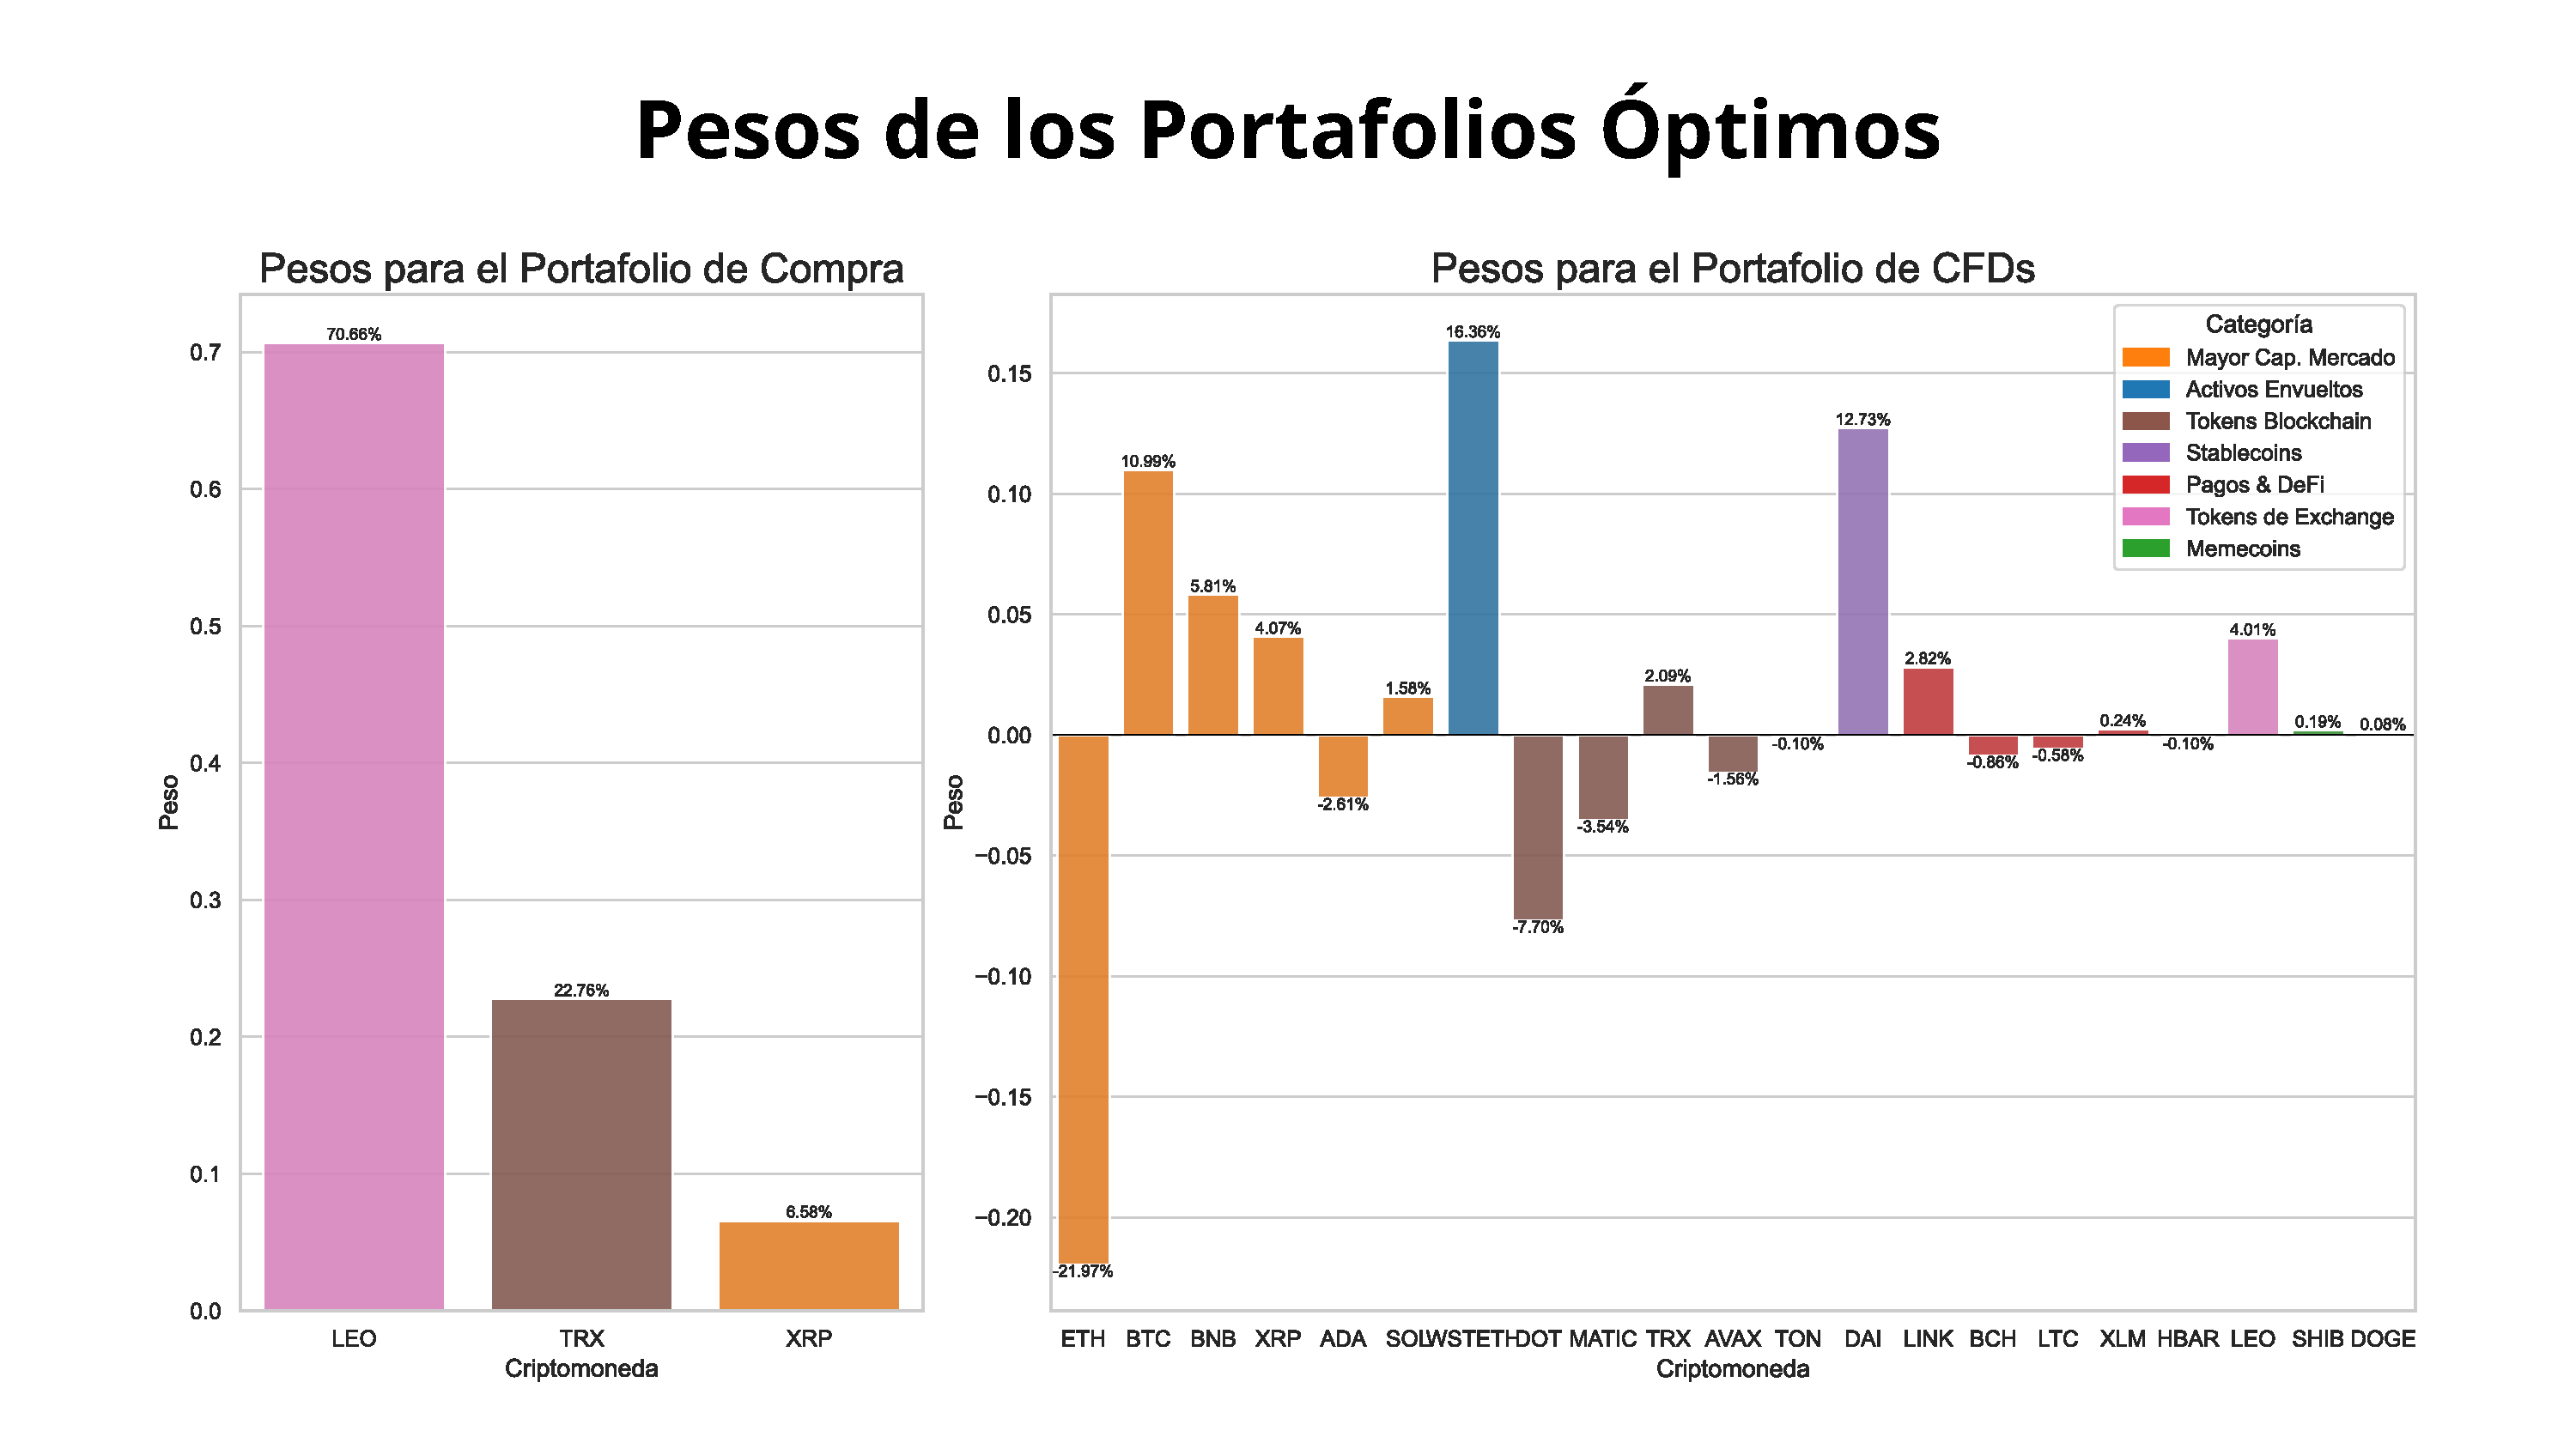
\includegraphics[width=0.8\textwidth]{imagenes/10-pesos.pdf}
    \caption{\textit{Elaboración Propia}. Descripción de la imagen.}
    \label{fig:peso}
\end{figure}

\section{Conclusiones y recomendaciones}

Los contratos por diferencia (CFDs) muestran retornos potenciales elevados, llegando a superar más del doble del margen, aunque acompañados de riesgos extremos, incluyendo escenarios de pérdida total del capital invertido.
El portafolio spot ofrece mayor estabilidad, siendo más adecuado para perfiles de inversión conservadores, llegando a 

\subsection{Recomendaciones estratégicas}
\begin{itemize}
\item Priorizar portafolios spot diversificados para horizontes temporales superiores a seis meses.
\item Implementar mecanismos de monitoreo dinámico de correlaciones y eventos relevantes con actualización periódica.
\item Reservar exposición a CFDs para perfiles con alta tolerancia al riesgo y experiencia en gestión activa de derivados.
\end{itemize}

\subsection{Limitaciones y propuestas futuras}
El modelo GBM asume normalidad y volatilidad constante, limitando su validez en contextos de alta heterocedasticidad o shocks extremos. Se proponen futuras investigaciones que:
\begin{itemize}
\item Incorporen modelos con saltos o volatilidad estocástica.
\item Amplíen el universo de activos incluyendo tokens DeFi, NFT, stablecoins algorítmicas y productos estructurados.
\item Integren modelos ARIMA-GARCH para captura de dependencias temporales y heterocedasticidad condicional.
\end{itemize}









\section{Referencias}

\begin{thebibliography}{99}
    \bibitem{bitgo2025wrapped}
    BitGo. (2025). \textit{Wrapped Bitcoin Documentation}. \url{https://www.bitgo.com}

    \bibitem{chainalysis2024crime}
    Chainalysis. (2024). \textit{Crypto Crime Report}. \url{https://www.chainalysis.com/reports/2024-crypto-crime-report/}

    \bibitem{coindesk2025xrp}
    CoinDesk. (2025). \textit{XRP Price Volatility Amid SEC Lawsuit Developments}. \url{https://www.coindesk.com/markets/2025/04/10/xrp-price-volatility-amid-sec-lawsuit/}

    \bibitem{coingecko2025marketcap}
    CoinGecko. (2025). \textit{Cryptocurrency Market Capitalizations}. \url{https://www.coingecko.com}

    \bibitem{coinmarketcap2025global}
    CoinMarketCap. (2025). \textit{Global Crypto Market Cap}. \url{https://www.coinmarketcap.com}

    \bibitem{cont2001empirical}
    Cont, R. (2001). Empirical properties of asset returns: stylized facts and statistical issues. \textit{Quantitative Finance, 1}(2), 223–236. \url{https://doi.org/10.1080/713665670}

    \bibitem{defillama2025tvl}
    DeFiLlama. (2025). \textit{DeFi Protocol Rankings by TVL}. \url{https://defillama.com}

    \bibitem{electriccapital2025developer}
    Electric Capital. (2025). \textit{Developer Report}. \url{https://www.electriccapital.com/developer-report}

    \bibitem{ethereumfoundation2024roadmap}
    Ethereum Foundation. (2024). \textit{Ethereum 2.0 Roadmap}. \url{https://ethereum.org/en/upgrades/}

    \bibitem{fidelity2025adoption}
    Fidelity Digital Assets. (2025). \textit{Institutional Crypto Adoption}. \url{https://www.fidelitydigitalassets.com/research}

    \bibitem{fisch2019disruptive}
    Fisch, C., Sandner, P., \& Schulte, P. (2019). Disruptive technology in the financial services industry: The case of blockchain-based ICOs. \textit{Technological Forecasting and Social Change, 136}, 118–130. \url{https://doi.org/10.1016/j.techfore.2018.09.020}

    \bibitem{hull2015options}
    Hull, J. C. (2015). \textit{Options, Futures, and Other Derivatives} (9th ed.). Pearson.

    \bibitem{kenett2010dominating}
    Kenett, D. Y., Tumminello, M., Madi, A., Gur-Gershgoren, G., Mantegna, R. N., \& Ben-Jacob, E. (2010). Dominating clasp of the financial sector revealed by partial correlation analysis of the stock market. \textit{PLoS ONE, 5}(12), e15032. \url{https://doi.org/10.1371/journal.pone.0015032}

    \bibitem{liu2022common}
    Liu, Y., Tsyvinski, A., \& Wu, X. (2022). Common risk factors in cryptocurrency. \textit{Journal of Finance, 77}(2), 1133–1177. \url{https://doi.org/10.1111/jofi.13039}

    \bibitem{makerdao2024dai}
    MakerDAO. (2024). \textit{DAI Stablecoin System Overview}. \url{https://makerdao.com/en/whitepaper/}

    \bibitem{mantegna1999hierarchical}
    Mantegna, R. N. (1999). Hierarchical structure in financial markets. \textit{European Physical Journal B, 11}, 193–197. \url{https://doi.org/10.1007/s100510050929}

    \bibitem{markowitz1952portfolio}
    Markowitz, H. (1952). Portfolio selection. \textit{Journal of Finance, 7}(1), 77–91. \url{https://doi.org/10.2307/2975974}

    \bibitem{messari2025thesis}
    Messari. (2025). \textit{Annual Crypto Thesis Report}. \url{https://messari.io/report/crypto-theses-2025}

    \bibitem{reuters2025elon}
    Reuters. (2025). \textit{Elon Musk Tweets Drive DOGE Surge}. \url{https://www.reuters.com/technology/elon-musks-tweets-drive-dogecoin-price-surge-2025-03-17/}

    \bibitem{santiment2024social}
    Santiment. (2024). \textit{Social Trends in Crypto}. \url{https://app.santiment.net}

    \bibitem{tumminello2005tool}
    Tumminello, M., Aste, T., Di Matteo, T., \& Mantegna, R. N. (2005). A tool for filtering information in complex systems. \textit{Proceedings of the National Academy of Sciences, 102}(30), 10421–10426. \url{https://doi.org/10.1073/pnas.0500298102}

    \bibitem{yahoofinance2025historical}
    Yahoo Finance. (2025). \textit{Cryptocurrency Historical Data}. \url{https://finance.yahoo.com}

    \bibitem{zhang2023cryptocurrency}
    Zhang, L., Zhang, X., \& Li, Y. (2023). Cryptocurrency Portfolio Construction: A Risk-Based Approach. \textit{Financial Innovation, 9}, 51. \url{https://doi.org/10.1186/s40854-023-00479-2}
\end{thebibliography}

\end{document}